\documentclass[12pt, a4paper]{article}

\title{\textsc{Logic Design} Lab 1: \textsf{\Large Fibonacci Number Detector}\\Report}
\author{110062219}
\date{\today}

\usepackage{amsmath}
\usepackage{amssymb}
\usepackage{caption}
\usepackage{subcaption}
\usepackage{circuitikz}
\usepackage{karnaugh-map}
\usepackage{float}
\usepackage{tikz}
\usetikzlibrary{graphs}
\usetikzlibrary{calc}

\begin{document}

\maketitle

\section{Design}

We are to carry out a 4-bit \textsf{Fibonacci Number Detector} in the Lab 1. It might be the most intuitive approach to adopt the \textbf{Behavaior Description}, in which we first enumerate all Fibonacci number less than 16 --- 0, 1, 2, 3, 5, 8, 13 --- and use \texttt{always} and \texttt{case} blocks to detect them.

\subsection{Karnaugh Map}

Since we are interested in hardware, we could take a further and more deep look at the logic and Boolean algebra.

\begin{figure}[htbp]
\begin{center}
\begin{karnaugh-map}[4][4][1][$i_1i_0$][$i_3i_2$]
\minterms{0, 1, 2, 3, 5, 8, 13}
\implicant{0}{2}
\implicant{5}{13}
\implicantedge{0}{0}{8}{8}
\end{karnaugh-map}
\caption{Karnaugh Map}
\label{kmap}
\end{center}
\end{figure}

The 4-bit integer input could be consider to be a 4 bits array $i_3i_2i_1i_0$. Then our detector $f$ could be write as sum of minterms $\sum{m(0, 1, 2, 3, 5, 8, 13)}$. By the means of \textit{Karnaugh Map} (Figure \ref{kmap}), we could select the implicants (red for $i_3'i_2'$, green for $i_2i_1'i_0$ and yellow for $i_2'i_1'i_0'$) and simplify $$f=i_3'i_2'+i_2i_1'i_0+i_2'i_1'i_0'$$. As a consequence, we could have the module come in \textbf{Dataflow Description} method.

\vfill

\subsection{Circuit Diagram}

If we would like to make our module more concrete, then we could draw the circuit diagram like Figure \ref{cd} based on the K-map and implement the module by \textbf{Gateway-level Description}.

\vfill

\begin{figure}[htbp]
\begin{center}
\begin{circuitikz}

\node[not port] (not a) at (-4, 4) {};
\node[not port] (not b) at (-4, 1.5) {};
\node[not port] (not c) at (-4, -1.5) {};
\node[not port] (not d) at (-4, -4) {};

\node[and port] (and 0) at (0, 3) {};
\node[and port, number inputs=3] (and 1) at (0, 0) {};
\node[and port, number inputs=3] (and 2) at (0, -3) {};

\node[or port, number inputs=3] (or) at (4, 0) {};

\draw (not a.in) -- ++(-2, 0) node[left] (a) {$i_3$};
\draw (not b.in) -- ++(-2, 0) node[left] (b) {$i_2$};
\draw (not c.in) -- ++(-2, 0) node[left] (c) {$i_1$};
\draw (not d.in) -- ++(-2, 0) node[left] (d) {$i_0$};

\draw (not a.out) -| (and 0.in 1);
\draw (not b.out) -| (and 0.in 2);

\draw (b) ++(.45,0) to[short,-*] ++(.55,0) |- (and 1.in 1);
\draw (d) ++(.45,0) to[short,-*] ++(.55,0) |- (and 1.in 2);
\draw (not c.out) -| (and 1.in 3);

\draw (not b.out) ++(.25,0) to[short,-*] ++(.35,0) |- (and 2.in 2);
\draw (not c.out) ++(.9,0) to[short,-*] ++(1,0) -| (and 2.in 1);
\draw (not d.out) -| (and 2.in 3);

\draw (and 0.out) -| (or.in 1);
\draw (and 1.out) -| (or.in 2);
\draw (and 2.out) -| (or.in 3);

\end{circuitikz}
\caption{Circuit Diagram}
\label{cd}
\end{center}
\end{figure}

\vfill

\subsection{Result}

In addition to the test bench module alone, I wrote a helper module which take $i$ and the outputs of each type of detectors as input and determine whether the output is either unknown or high impendence, or the output is conflict with the fact so that the condition we check is more clear.

Figure \ref{ss} shows the result of \texttt{ncverilog}.

\begin{figure}[htbp]
\begin{center}
\centering
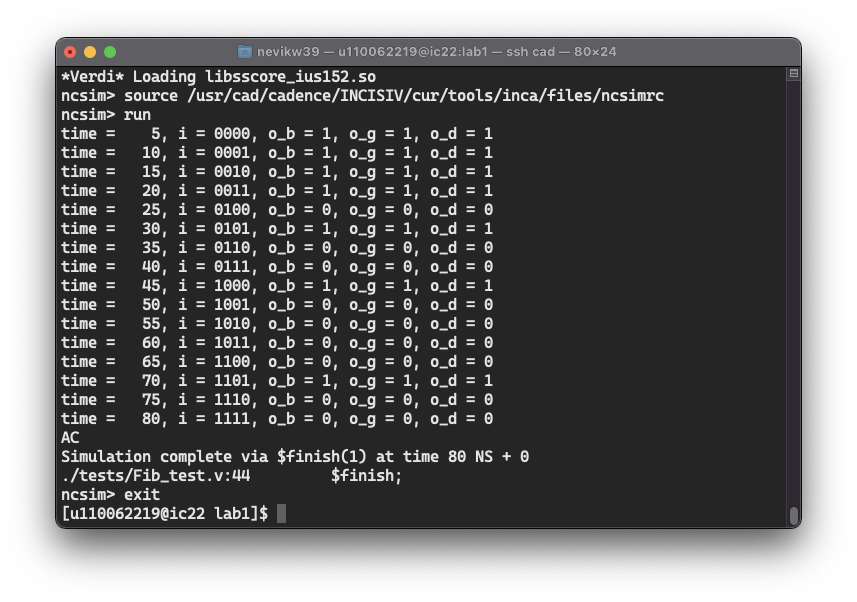
\includegraphics[width=\textwidth]{screenshot}
\caption{Screenshot}
\label{ss}
\end{center}
\end{figure}

\section{Problems}

Since it was my very first time to write \textit{Verilog}, it's inevitable and natural that I encountered several problems.

In the beginning, I ran into the problem that I wanted to use the remote SSH feature of VS Code, but \texttt{ncverilog} is at the node inside the CAD server. After searching some resources, I found out how to configure so that I could connect to the node via CAD server as a proxy jump server.

Moreover, it seemed that some environment variables weren't set properly when connecting through VS Code. I tried to override the \texttt{\$PATH} manually and switch to \texttt{bash}, and it worked sometimes, but \texttt{ncverilog} got license failed once in a while. After searching some resources, I found out it's because VS Code use \texttt{bash} as default and not run \texttt{.profile} properly, so I returned to default shell \texttt{tcsh} and select it as the default terminal of VS Code.

Last but not least, I had some difficult time to draw the circuit diagram (Figure \ref{cd}) in \LaTeX, though to draw the K-map was much more easy.
\section{Reflection}

I really learnt a lot in this Lab. To begin with, I wrote my debut \textit{Verilog} codes and learnt its fundamental again in a more comprehensive and practical view.

Furthermore, I acquired more knowledge about SSH and Linux shell. Although it's hard to draw the circuit diagram in \LaTeX, I'm quite satisfied with my result, which gives me a sense of accomplishment.

In the end, since there's no solid and definite specification on the report, so I'm not sure if my format is acceptable.

\end{document}
